\section{MGnify samples benchmark}\label{sec:MGnify's samples}
\subsection{Benchmark of Galaxy-ported rRNA-prediction subworkflow pipeline against its MGnify counterpart}\label{subsec:mgnifyVSgalaxy}
The results for the benchmark of samples from two different biomes, human large intestine and soil, are shown in \Cref{fig:mgnify_human_gut_beta_div,fig:mgnify_soil_beta_div}. These figures provide a graphical presentation of dissimilarity values computed using the two metrics, Bray Curtis distance and Jaccard distance, at each taxonomic rank, as well as for all ranks combined.
Two trends can be observed in the beta diversity plots (\Cref{fig:mgnify_human_gut_beta_div,fig:mgnify_soil_beta_div}). First, lower taxonomic ranks show on average, higher dissimilarity values than higher ranks. In both MGnify and Galaxy-port results, the taxonomic ranks of super kingdom and kingdom exhibited identical taxa presence (Jaccard distance equals 0) and nearly identical abundance (Bray Curtis distance of approximately 0). The highest average dissimilarity values were observed at the species rank. The second notable trend involves Jaccard distance values being consistently greater than the Bray Curtis values, from the phylum rank downwards. The second trend was caused by individual taxa having an abundance of 1 in MGnify's results while being absent in Galaxy's results, or vice versa (see example in \Cref{jaccard_example}).
\begin{figure}[H]
  \centering
  \hfill
  \subfloat{{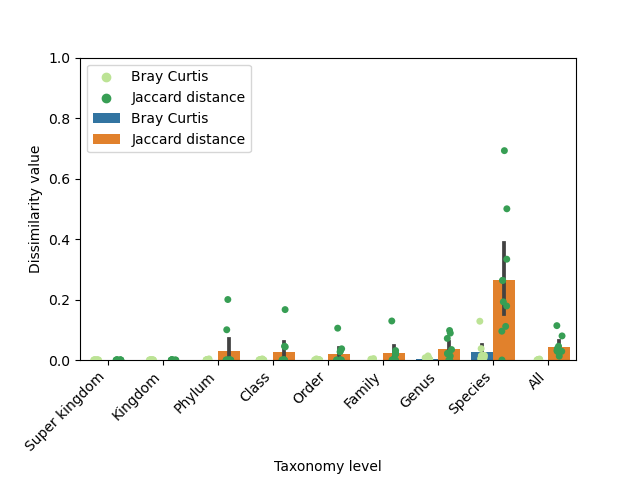
\includegraphics[scale=0.8]{figures/human_gut_plot_galaxyVSmgnify.png} }}%
  \captionof{figure}[Beta diversity-based benchmark. Dissimilarity between MGnify and Galaxy-ported pipeline, for MGnify human large intestine samples]{\textbf{Beta diversity-based benchmark}. Dissimilarity between MGnify and Galaxy-ported pipeline, for MGnify human large intestine samples (\Cref{tab:human-gut-samples}). The term 'All' refers to all ranks combined. Bars represent the average dissimilarity values, while individual data points represent the values for each of the individual samples.} \label{fig:mgnify_human_gut_beta_div}%
\end{figure}

\begin{figure}[H]
  \centering
  \hfill
  \subfloat{{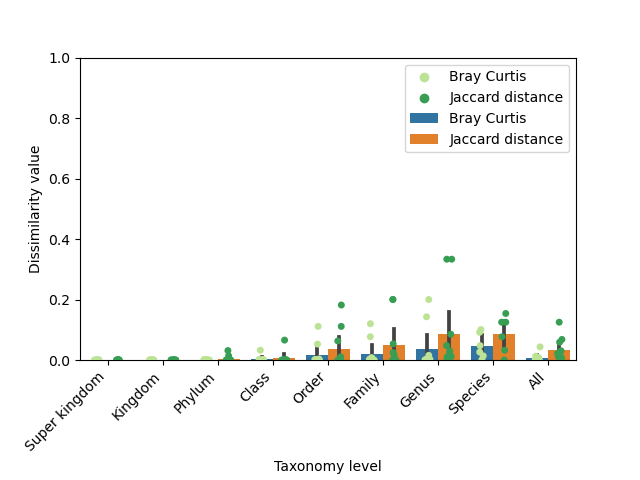
\includegraphics[scale=0.8]{figures/soil_plot_galaxyVSmgnify.png} }}%
  \captionof{figure}[Beta diversity-based benchmark. Dissimilarity between MGnify and Galaxy-ported pipeline, for MGnify soil samples]{\textbf{Beta diversity-based benchmark}. Dissimilarity between MGnify and Galaxy-ported pipeline, for MGnify soil samples (\Cref{tab:soil-samples}). The term 'All' refers to all ranks combined. Bars represent the average dissimilarity values, while individual data points represent the values for each of the individual samples.} \label{fig:mgnify_soil_beta_div}%
\end{figure}
The relative abundance comparison, at genus and species ranks, for MGnify samples for two biomes, human large intestine and soil, is shown in \Cref{fig:mgnify_human_gut_rel_abundance_s_level,fig:mgnify_human_gut_rel_abundance_g_level,fig:mgnify_soil_rel_abundace_s_level,fig:mgnify_soil_rel_abundace_g_level}. Taxa in the output of Galaxy port different to MGnify were excluded to highlight the discrepancy in the resulting plots.
The relative abundance plots (\Cref{fig:mgnify_human_gut_rel_abundance_s_level,fig:mgnify_human_gut_rel_abundance_g_level,fig:mgnify_soil_rel_abundace_s_level,fig:mgnify_soil_rel_abundace_g_level}) show overall good agreement of similarity for taxa with high relative abundance for both of the genus and species ranks. Additionally, in these charts, the Galaxy visual representation showed only isolated small gaps, which indicates only small quantities of taxa were present in Galaxy-port results, yet absent in the MGnify results.\\
The relative abundance plot for soil at the species rank (\Cref{fig:mgnify_soil_rel_abundace_s_level}) concluded only six of the ten benchmarked soil samples. The four absent samples, corresponding to the analyses MGYA00553054, MGYA00578739, MGYA00578910, and MGYA00578954, did not contain any reads at the species rank in either the MGnify or Galaxy-ported results.\\

\begin{figure}[H]
  \centering
  \subfloat{{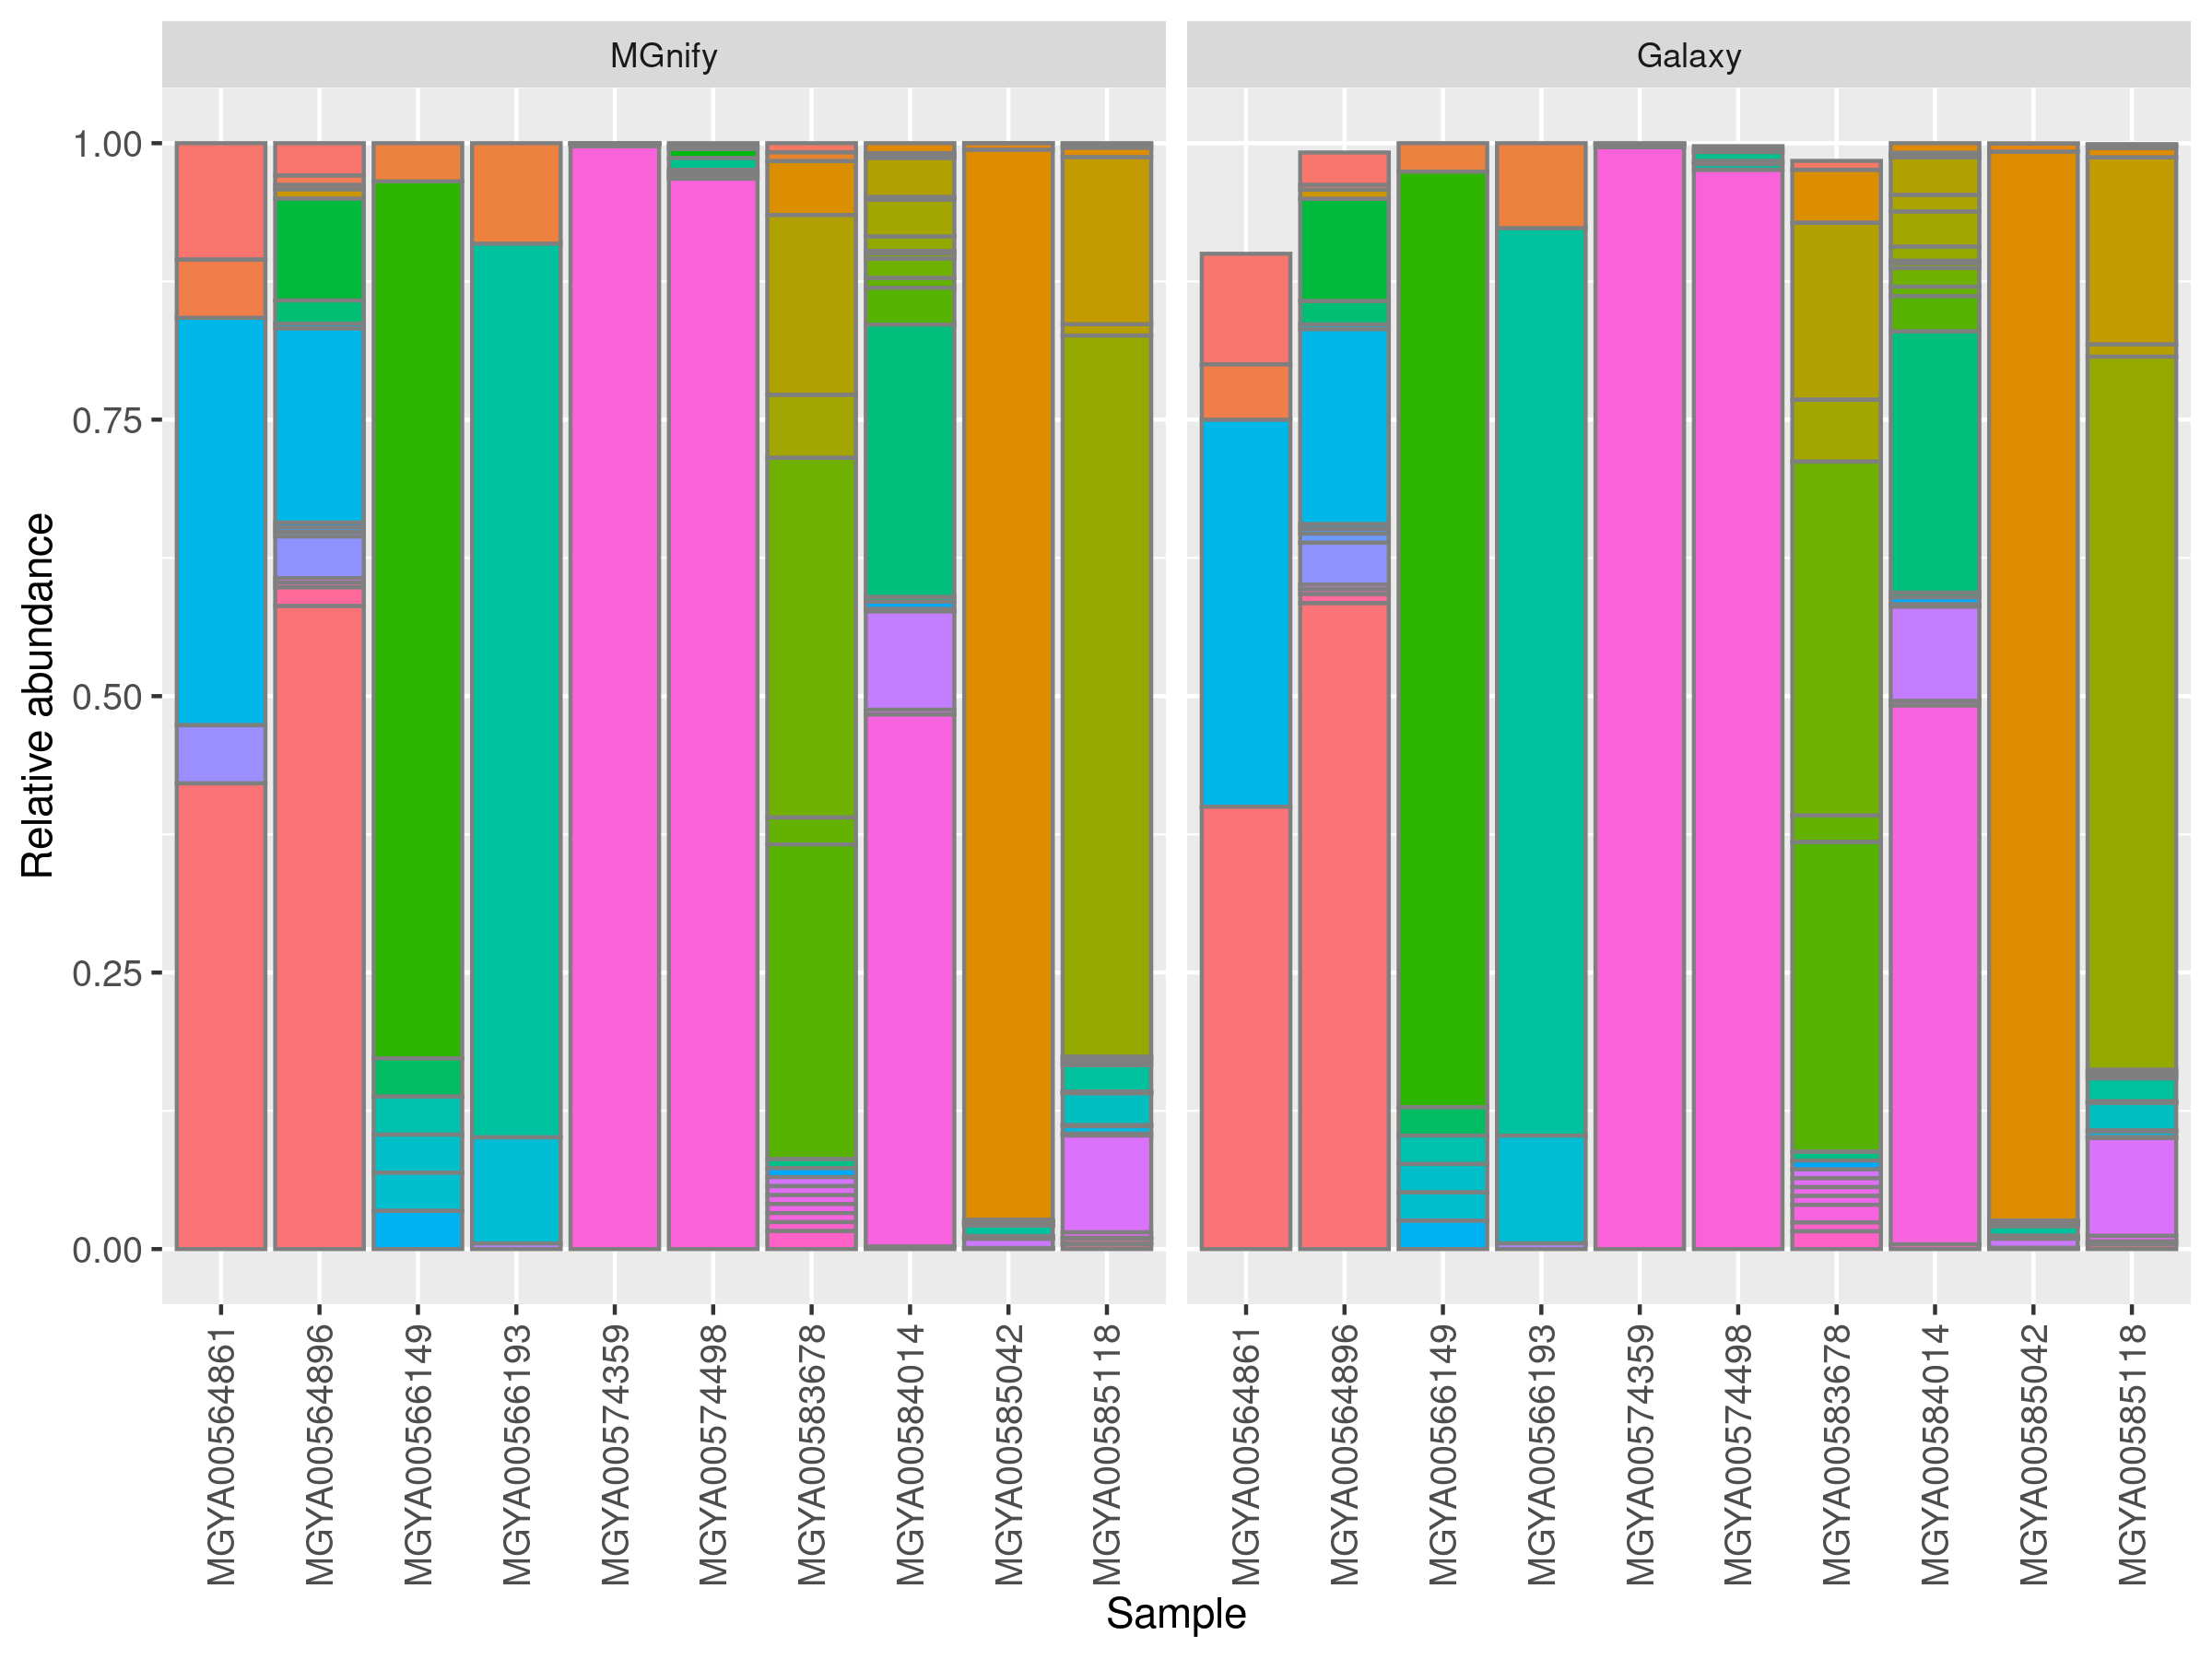
\includegraphics[scale=0.65]{figures/human_gut_abundance_level_s_mgnifyVSgalaxy.png} }}%
  \captionof{figure}[Differences of relative abundance between MGnify and Galaxy-ported pipeline at species rank for MGnify human large intestine samples]{\textbf{Differences of relative abundance between MGnify and Galaxy-ported pipeline at species rank for MGnify human large intestine samples}~(\Cref{tab:human-gut-samples}). Species that were predicted by Galaxy but were not present in the MGnify output are not shown. The plot legend can be found in the appendix (\Cref{fig:human_gut_abundance_level_s_mgnifyVSgalaxy_legend.png})} \label{fig:mgnify_human_gut_rel_abundance_s_level}%
\end{figure}

\begin{figure}[H]
  \centering
  \subfloat{{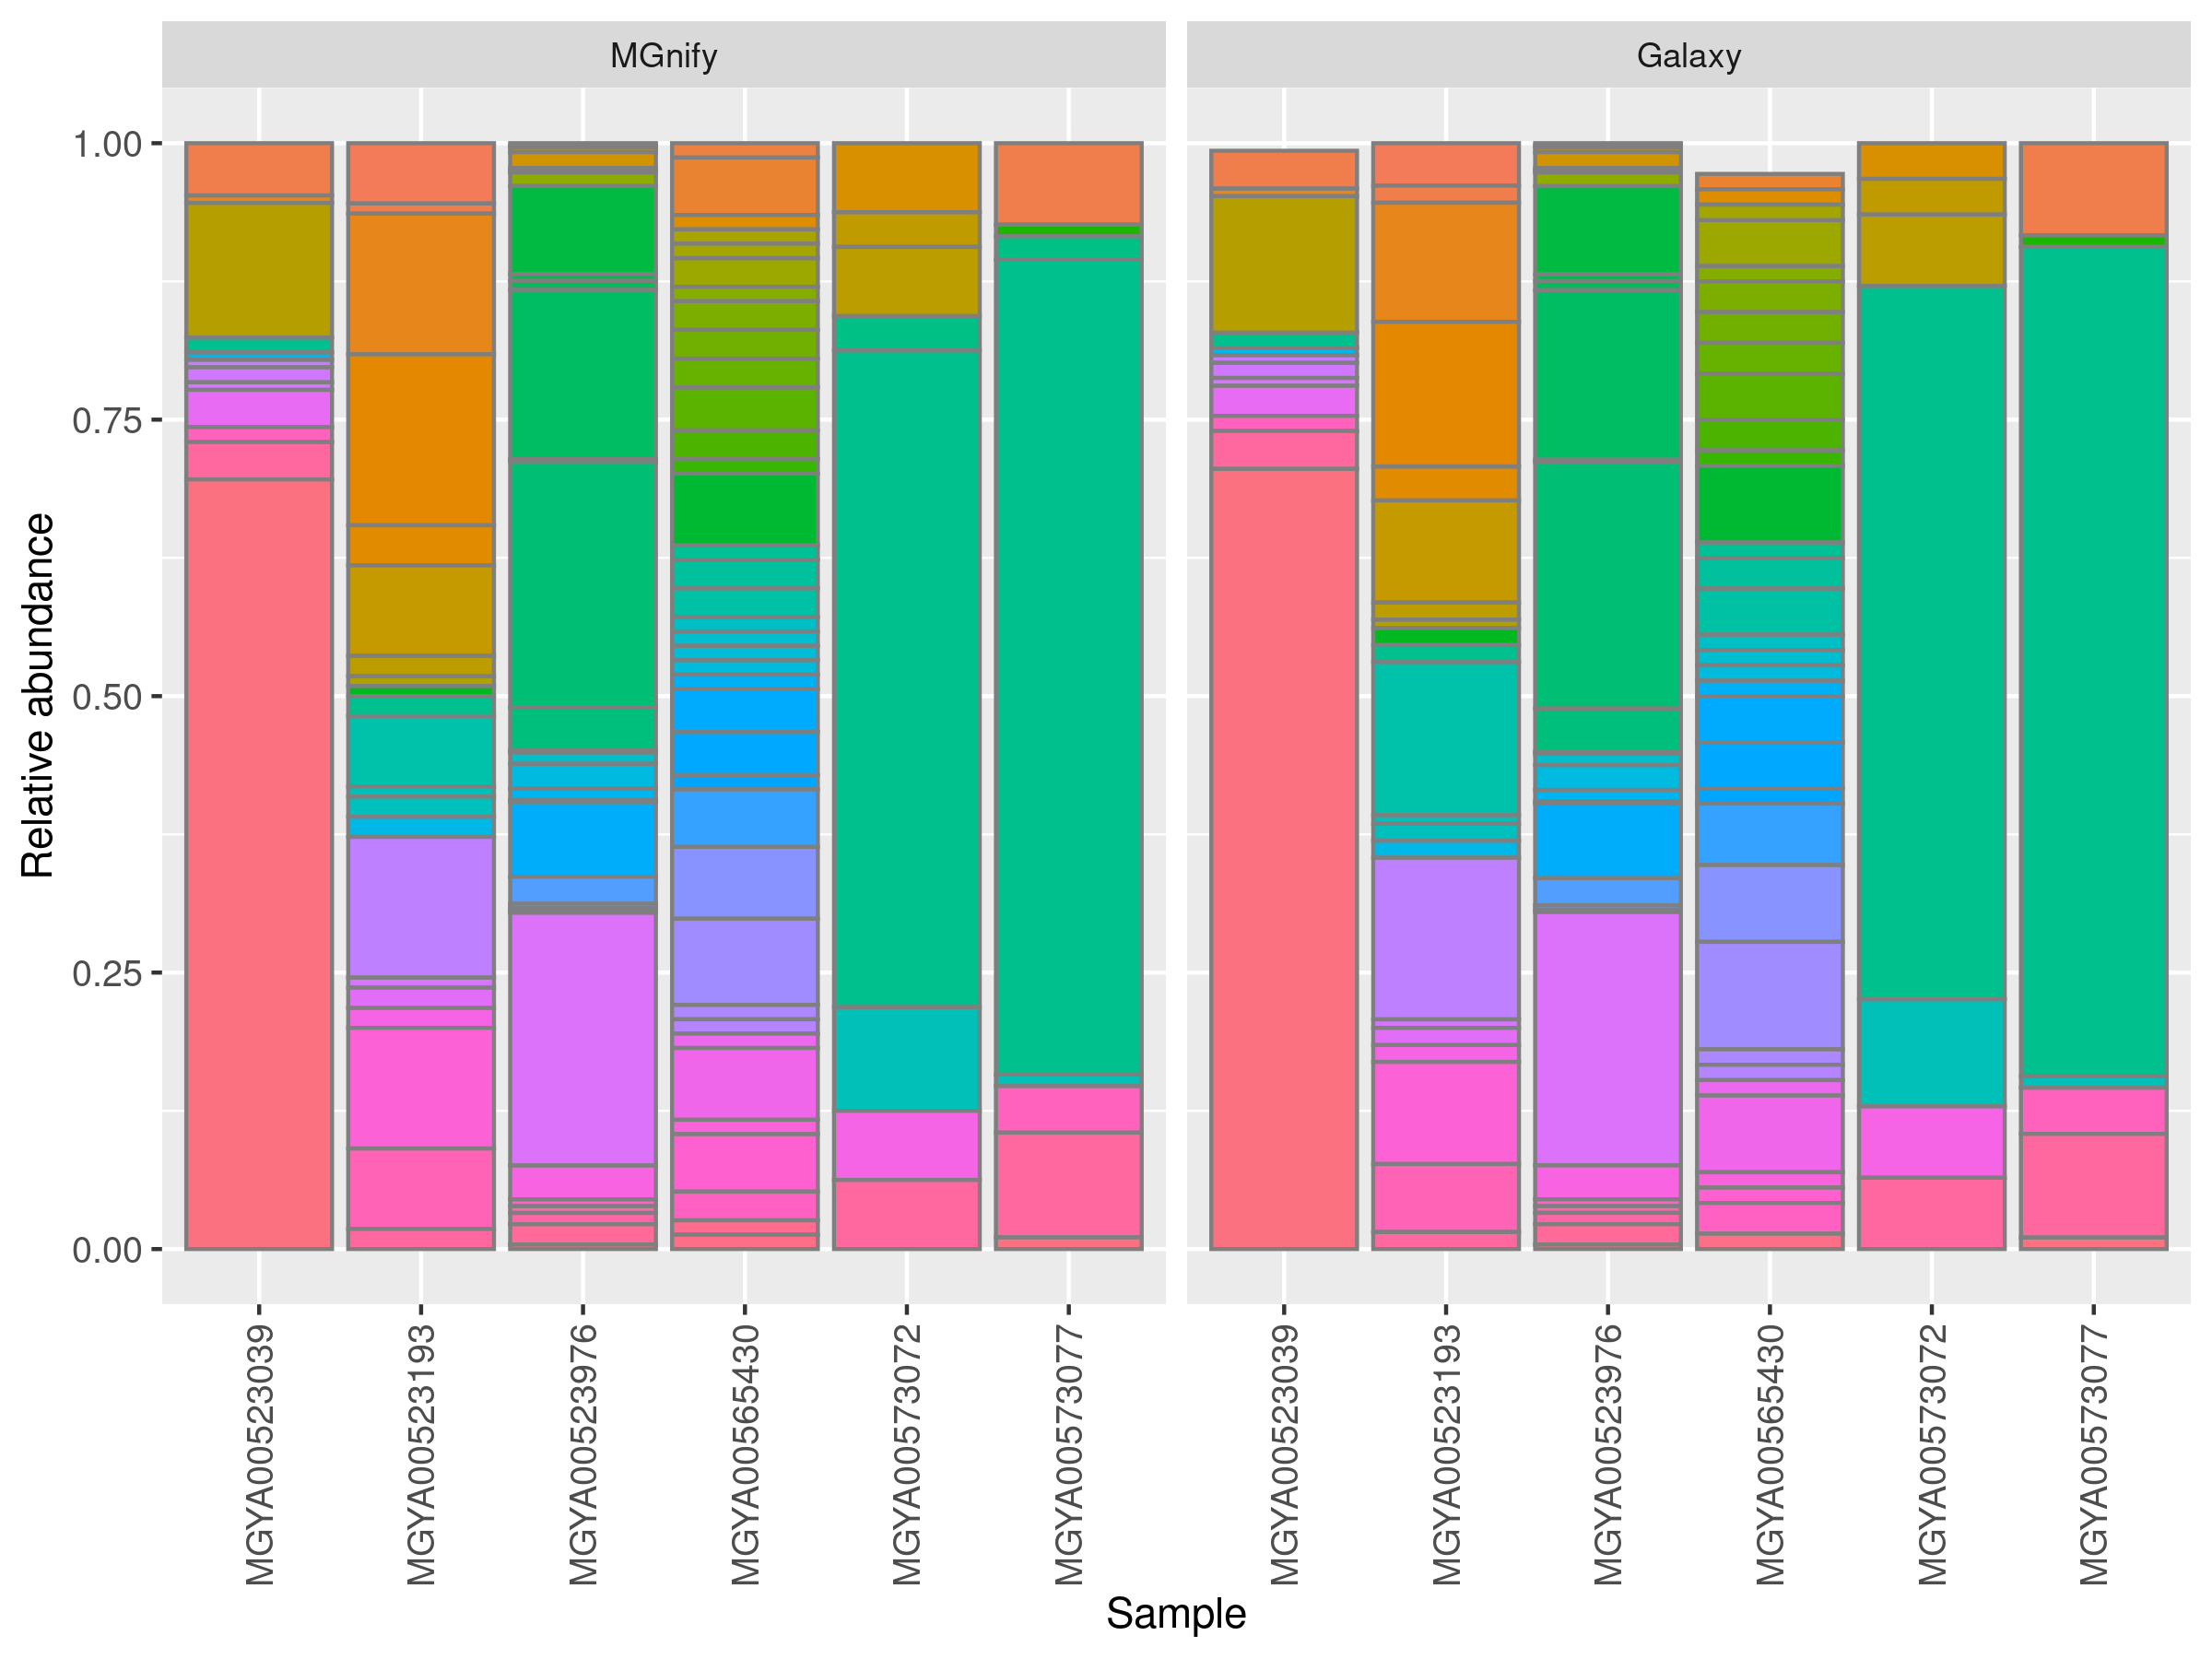
\includegraphics[scale=0.65]{figures/soil_abundace_level_s_mgnifyVSgalaxy.png} }}%
  \captionof{figure}[Differences of relative abundance between MGnify and Galaxy-ported pipeline at species rank for MGnify soil samples]{\textbf{Differences of relative abundance between MGnify and Galaxy-ported pipeline at species rank for MGnify soil samples}(\Cref{tab:soil-samples}). Species that were predicted by Galaxy but not present in the MGnify output are not shown. Some samples did not include any reads for the species rank. The plot legend can be found in the appendix (\Cref{fig:soil_abundace_level_s_mgnifyVSgalaxy_legend.png})} \label{fig:mgnify_soil_rel_abundace_s_level}%
\end{figure}

\begin{figure}[H]
  \centering
  \subfloat{{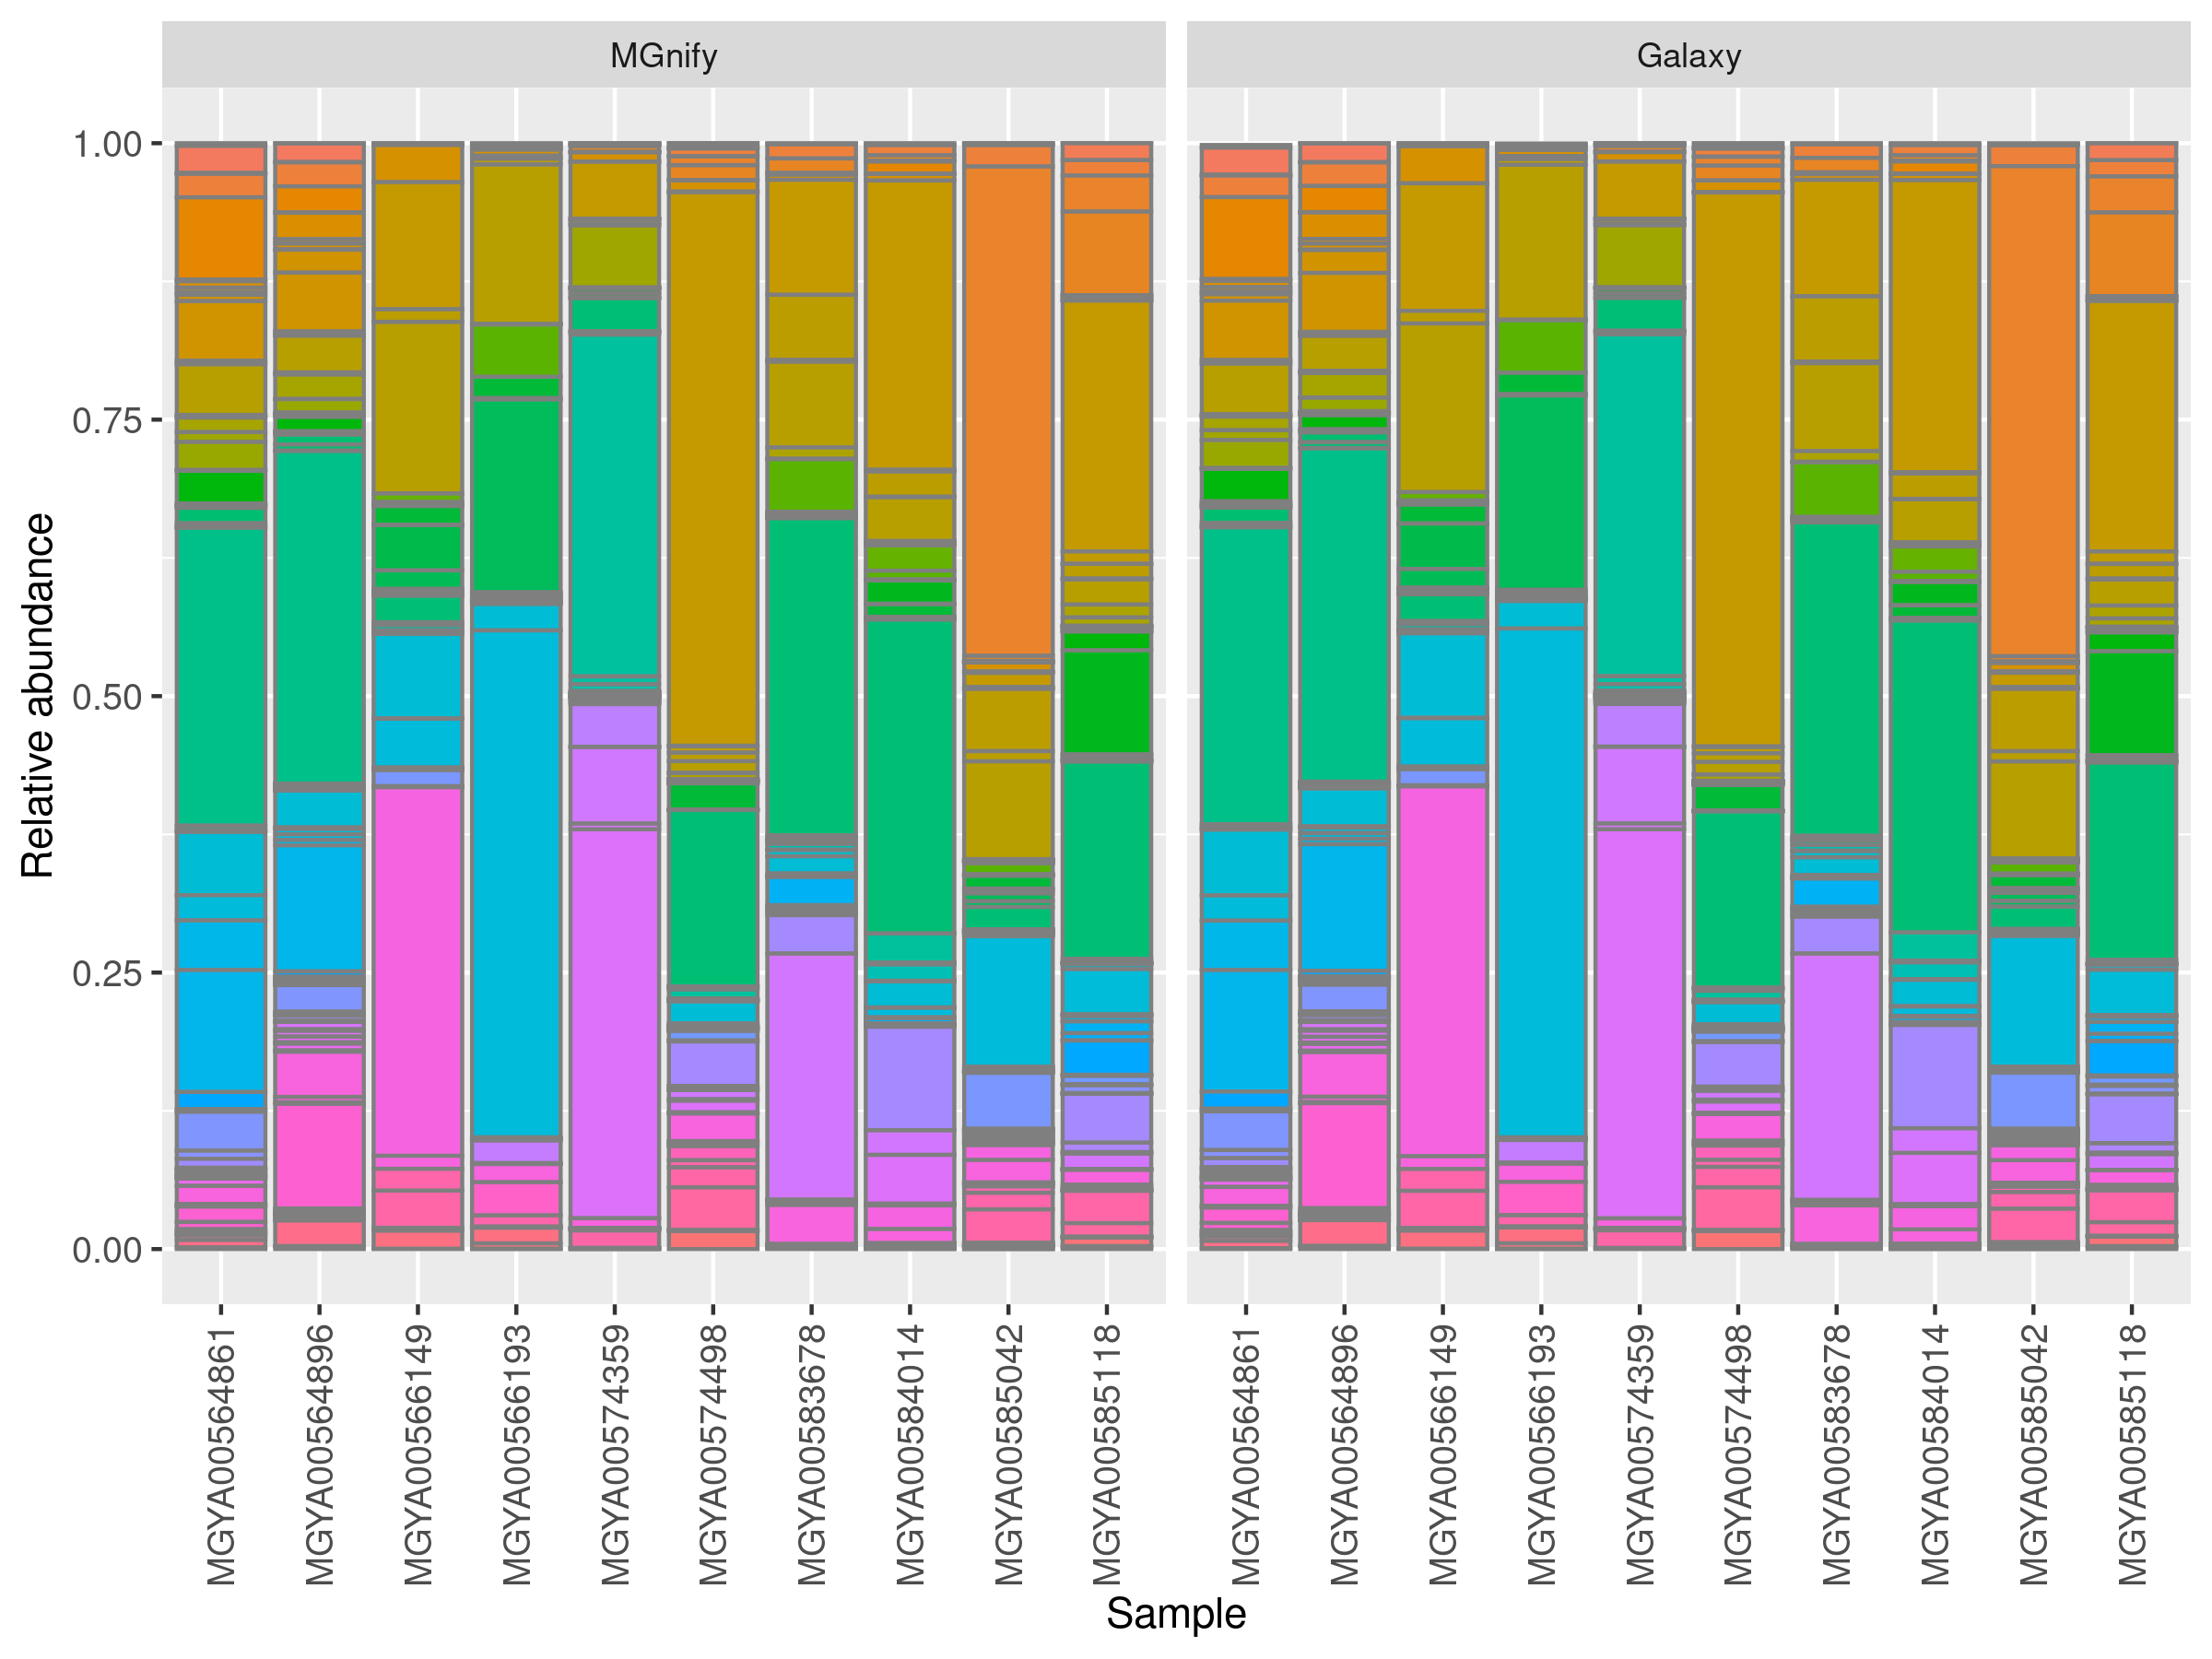
\includegraphics[scale=0.7]{figures/human_gut_abundance_level_g_mgnifyVSgalaxy.png} }}%
  \captionof{figure}[Differences of relative abundance between MGnify and Galaxy-ported pipeline at genus rank for MGnify human large intestine samples]{\textbf{Differences of relative abundance between MGnify and Galaxy-ported pipeline at genus rank for MGnify human large intestine samples}(\Cref{tab:human-gut-samples}). Genera that were predicted by Galaxy but not present in the MGnify output are not shown. The plot legend can be found in the appendix (\Cref{fig:human_gut_abundance_level_g_mgnifyVSgalaxy_legend.png})} \label{fig:mgnify_human_gut_rel_abundance_g_level}%
\end{figure}

\begin{figure}[H]
  \centering
  \subfloat{{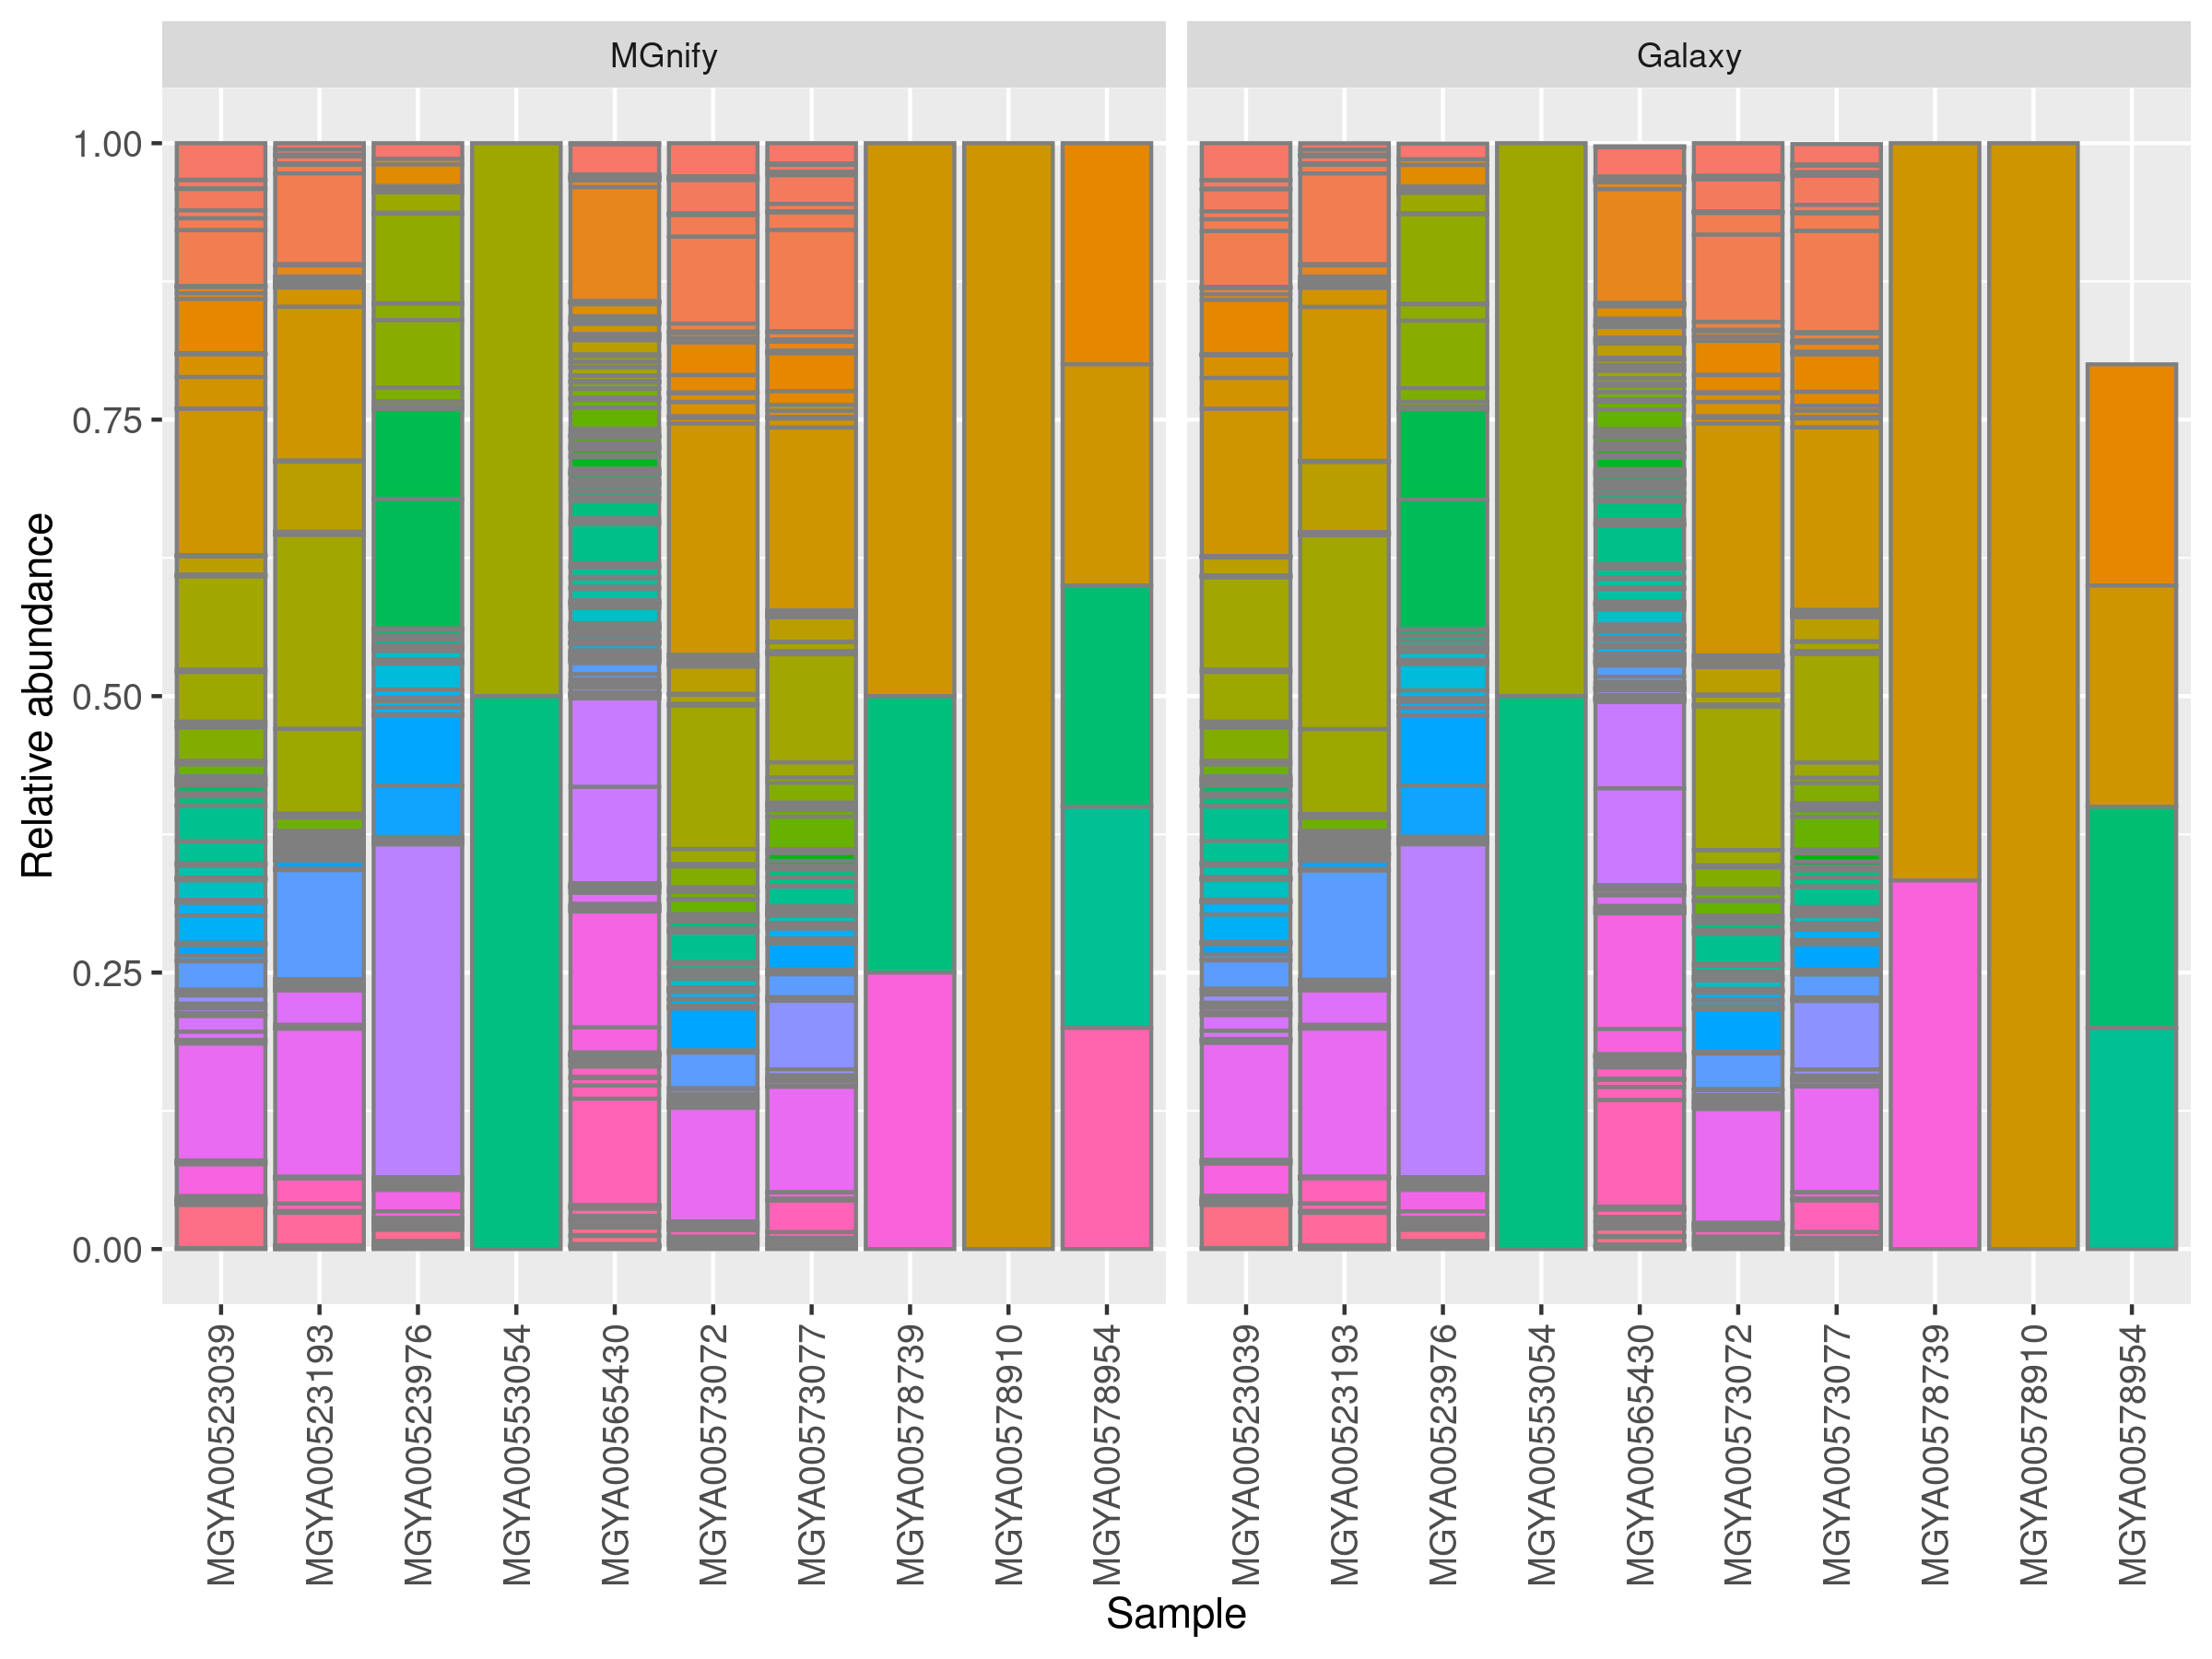
\includegraphics[scale=0.7]{figures/soil_abundance_level_g_mgnifyVSgalaxy.png} }}%
  \captionof{figure}[Differences of relative abundance between MGnify and Galaxy-ported pipeline at genus rank for MGnify soil samples]{\textbf{Differences of relative abundance between MGnify and Galaxy-ported pipeline at genus rank for MGnify soil samples}(\Cref{tab:soil-samples}). Genera that were predicted by Galaxy but not present in the MGnify output are not shown. The plot legend can be found in the appendix (\Cref{fig:soil_abundance_level_g_mgnifyVSgalaxy_legend.png})} \label{fig:mgnify_soil_rel_abundace_g_level}%
\end{figure}


\subsection{Benchmark of Kraken v2 against MGnify rRNA-prediction subworkflow}\label{subsec:mgnifyVSkraken2}
For the comparison between MGnify and Kraken v2, it was necessary to exclude the super kingdom and species ranks from MGnify results. Additionally, adjustments were made to the kingdom rank, to match the Kraken v2 taxonomic lineage.\\
The beta diversity plots (\Cref{fig:human_gut_plot_mgnifyVSkraken2.png,fig:soil_plot_mgnifyVSkraken2.png}) show overall high average dissimilarity values. Additionally, the average Jaccard distance values consistently exceeded the average Bray Curtis distance values. These substantial dissimilarities are also noticeable in the generated relative abundance plots for the genus rank (\Cref{fig:human_large_intestine_rel_abundance_mgnifyVSkraken2,fig:soil_rel_abundance_mgnifyVSkraken2}), where significant gaps in the Kraken v2 visual representation indicate a high relative abundance of detected taxa that are absent in MGnify results, especially within the soil samples.\\

\begin{figure}[H]
  \centering
  \hfill
  \subfloat{{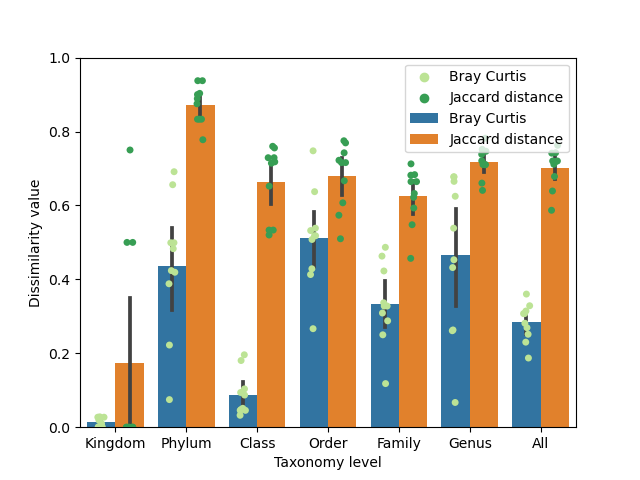
\includegraphics[scale=0.8]{figures/human_gut_plot_mgnifyVSkraken2.png} }}%
  \captionof{figure}[Beta diversity-based benchmark.Dissimilarity between MGnify and Kraken v2, for the MGnify human large intestine samples]{\textbf{Beta diversity-based benchmark}. Dissimilarity between MGnify and Kraken v2, for the MGnify human large intestine samples (\Cref{tab:human-gut-samples}) The term 'All' refers to all ranks combined. Bars represent the average dissimilarity values, while individual data points represent the values for each of the individual samples.} \label{fig:human_gut_plot_mgnifyVSkraken2.png}%
\end{figure}
\begin{figure}[H]
  \centering
  \hfill
  \subfloat{{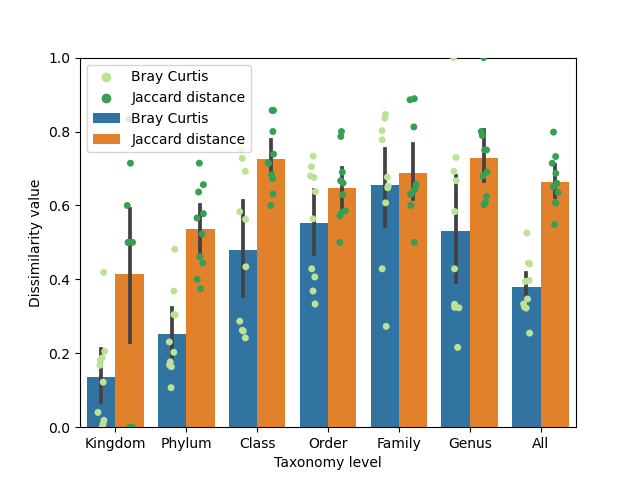
\includegraphics[scale=0.8]{figures/soil_plot_mgnifyVSkraken2.png} }}%
  \captionof{figure}[Beta diversity-based benchmark. Dissimilarity between MGnify and Kraken v2, for MGnify soil samples]{\textbf{Beta diversity-based benchmark}. Dissimilarity between MGnify and Kraken v2, for MGnify soil samples (\Cref{tab:soil-samples}). The term 'All' refers to all ranks combined. Bars represent the average dissimilarity values, while individual data points represent the values for each of the individual samples.}
  \label{fig:soil_plot_mgnifyVSkraken2.png}%
\end{figure}